% ------------------------------------------------------------
% LaTeX Template für die DHBW zum Schnellstart!
% Original: https://github.wdf.sap.corp/vtgermany/LaTeX-Template-DHBW
% ------------------------------------------------------------
% ---- Präambel mit Angaben zum Dokument
\documentclass[
	fontsize=12pt,           % Leitlinien sprechen von Schriftgröße 12.
	paper=A4,
	twoside=false,
	listof=totoc,            % Tabellen- und Abbildungsverzeichnis ins Inhaltsverzeichnis
	bibliography=totoc,      % Literaturverzeichnis ins Inhaltsverzeichnis aufnehmen
	titlepage,               % Titlepage-Umgebung anstatt \maketitle
	headsepline,             % horizontale Linie unter Kolumnentitel
	abstract,              % Überschrift einschalten, Abstract muss in {abstract}-Umgebung stehen
]{scrreprt}                  % Verwendung von KOMA-Report
\usepackage[utf8]{inputenc}  % UTF8 Encoding einschalten
\usepackage[ngerman]{babel}  % Neue deutsche Rechtschreibung
\usepackage[T1]{fontenc}     % Ausgabe von westeuropäischen Zeichen (auch Umlaute)
\usepackage{microtype}       % Trennung von Wörtern wird besser umgesetzt
\usepackage{lmodern}         % Nicht-gerasterte Schriftarten (bei MikTeX erforderlich)
\usepackage{graphicx}        % Einbinden von Grafiken erlauben
\usepackage{wrapfig}         % Grafiken fließend im Text
\usepackage{setspace}        % Zeilenabstand \singlespacing, \onehalfspaceing, \doublespacing
\usepackage[
	%showframe,                % Ränder anzeigen lassen
	left=2.7cm, right=2.5cm,
	top=2.5cm,  bottom=2.5cm,
	includeheadfoot
]{geometry}                      % Seitenlayout einstellen
\usepackage{scrlayer-scrpage}    % Gestaltung von Fuß- und Kopfzeilen
\usepackage{acronym}             % Abkürzungen, Abkürzungsverzeichnis
\usepackage{titletoc}            % Anpassungen am Inhaltsverzeichnis
\contentsmargin{0.75cm}          % Abstand im Inhaltsverzeichnis zw. Punkt und Seitenzahl
\usepackage[                     % Klickbare Links (enth. auch "nameref", "url" Package)
  hidelinks,                     % Blende die "URL Boxen" aus.
  breaklinks=true                % Breche zu lange URLs am Zeilenende um
]{hyperref}
\usepackage[hypcap=true]{caption}% Anker Anpassung für Referenzen
\urlstyle{same}                  % Aktuelle Schrift auch für URLs
% Anpassung von autoref für Gleichungen (ergänzt runde Klammern) und Algorithm.
% Anstatt "Listing" kann auch z.B. "Code-Ausschnitt" verwendet werden. Dies sollte
% jedoch synchron gehalten werden mit \lstlistingname (siehe weiter unten).
\addto\extrasngerman{%
	\def\equationautorefname~#1\null{Gleichung~(#1)\null}
	\def\lstnumberautorefname{Zeile}
	\def\lstlistingautorefname{Listing}
	\def\algorithmautorefname{Algorithmus}
	% Damit einheitlich "Abschnitt 1.2[.3]" verwendet wird und nicht "Unterabschnitt 1.2.3"
	% \def\subsectionautorefname{Abschnitt}
}

% ---- Abstand verkleinern von der Überschrift 
\renewcommand*{\chapterheadstartvskip}{\vspace*{.5\baselineskip}}

% Hierdurch werden Schusterjungen und Hurenkinder vermieden, d.h. einzelne Wörter
% auf der nächsten Seite oder in einer einzigen Zeile.
% LaTeX kann diese dennoch erzeugen, falls das Layout ansonsten nicht umsetzbar ist.
% Diese Werte sind aber gute Startwerte.
\widowpenalty10000
\clubpenalty10000

% ---- Für das Quellenverzeichnis
\usepackage[
	backend = biber,                % Verweis auf biber
	language = auto,
	style = numeric,                % Nummerierung der Quellen mit Zahlen
	sorting = none,                 % none = Sortierung nach der Erscheinung im Dokument
	sortcites = true,               % Sortiert die Quellen innerhalb eines cite-Befehls
	block = space,                  % Extra Leerzeichen zwischen Blocks
	hyperref = true,                % Links sind klickbar auch in der Quelle
	%backref = true,                % Referenz, auf den Text an die zitierte Stelle
	bibencoding = auto,
	giveninits = true,              % Vornamen werden abgekürzt
	doi=false,                      % DOI nicht anzeigen
	isbn=false,                     % ISBN nicht anzeigen
    alldates=short                  % Datum immer als DD.MM.YYYY anzeigen
]{biblatex}
\addbibresource{Inhalt/literatur.bib}
\setcounter{biburlnumpenalty}{3000}     % Umbruchgrenze für Zahlen
\setcounter{biburlucpenalty}{6000}      % Umbruchgrenze für Großbuchstaben
\setcounter{biburllcpenalty}{9000}      % Umbruchgrenze für Kleinbuchstaben
\DeclareNameAlias{default}{family-given}  % Nachname vor dem Vornamen
\AtBeginBibliography{\renewcommand{\multinamedelim}{\addslash\space
}\renewcommand{\finalnamedelim}{\multinamedelim}}  % Schrägstrich zwischen den Autorennamen
\DefineBibliographyStrings{german}{
  urlseen = {Einsichtnahme:},                      % Ändern des Titels von "besucht am"
}
\usepackage[babel,german=quotes]{csquotes}         % Deutsche Anführungszeichen + Zitate


% ---- Für Mathevorlage
\usepackage{amsmath}    % Erweiterung vom Mathe-Satz
\usepackage{amssymb}    % Lädt amsfonts und weitere Symbole
\usepackage{MnSymbol}   % Für Symbole, die in amssymb nicht enthalten sind.


% ---- Für Quellcodevorlage
\usepackage{scrhack}                    % Hack zur Verw. von listings in KOMA-Script
\usepackage{listings}                   % Darstellung von Quellcode
\usepackage{xcolor}                     % Einfache Verwendung von Farben
% -- Eigene Farben für den Quellcode
\definecolor{JavaLila}{rgb}{0.4,0.1,0.4}
\definecolor{JavaGruen}{rgb}{0.3,0.5,0.4}
\definecolor{JavaBlau}{rgb}{0.0,0.0,1.0}
\definecolor{ABAPKeywordsBlue}{HTML}{6000ff}
\definecolor{ABAPCommentGrey}{HTML}{808080}
\definecolor{ABAPStringGreen}{HTML}{4da619}
\definecolor{PyKeywordsBlue}{HTML}{0000AC}
\definecolor{PyCommentGrey}{HTML}{808080}
\definecolor{PyStringGreen}{HTML}{008080}
% -- Farben für ABAP CDS
\definecolor{CDSString}{HTML}{FF8C00}
\definecolor{CDSKeywords}{HTML}{6000ff}
\definecolor{CDSAnnotation}{HTML}{00BFFF}
\definecolor{CDSComment}{HTML}{808080}
\definecolor{CDSFunc}{HTML}{FF0000}

% -- Default Listing-Styles

\lstset{
	% Das Paket "listings" kann kein UTF-8. Deswegen werden hier 
	% die häufigsten Zeichen definiert (ä,ö,ü,...)
	literate=%
		{á}{{\'a}}1 {é}{{\'e}}1 {í}{{\'i}}1 {ó}{{\'o}}1 {ú}{{\'u}}1
		{Á}{{\'A}}1 {É}{{\'E}}1 {Í}{{\'I}}1 {Ó}{{\'O}}1 {Ú}{{\'U}}1
		{à}{{\`a}}1 {è}{{\`e}}1 {ì}{{\`i}}1 {ò}{{\`o}}1 {ù}{{\`u}}1
		{À}{{\`A}}1 {È}{{\'E}}1 {Ì}{{\`I}}1 {Ò}{{\`O}}1 {Ù}{{\`U}}1
		{ä}{{\"a}}1 {ë}{{\"e}}1 {ï}{{\"i}}1 {ö}{{\"o}}1 {ü}{{\"u}}1
		{Ä}{{\"A}}1 {Ë}{{\"E}}1 {Ï}{{\"I}}1 {Ö}{{\"O}}1 {Ü}{{\"U}}1
		{â}{{\^a}}1 {ê}{{\^e}}1 {î}{{\^i}}1 {ô}{{\^o}}1 {û}{{\^u}}1
		{Â}{{\^A}}1 {Ê}{{\^E}}1 {Î}{{\^I}}1 {Ô}{{\^O}}1 {Û}{{\^U}}1
		{œ}{{\oe}}1 {Œ}{{\OE}}1 {æ}{{\ae}}1 {Æ}{{\AE}}1 {ß}{{\ss}}1
		{ű}{{\H{u}}}1 {Ű}{{\H{U}}}1 {ő}{{\H{o}}}1 {Ő}{{\H{O}}}1
		{ç}{{\c c}}1 {Ç}{{\c C}}1 {ø}{{\o}}1 {å}{{\r a}}1 {Å}{{\r A}}1
		{€}{{\euro}}1 {£}{{\pounds}}1 {«}{{\guillemotleft}}1
		{»}{{\guillemotright}}1 {ñ}{{\~n}}1 {Ñ}{{\~N}}1 {¿}{{?`}}1,
	breaklines=true,        % Breche lange Zeilen um 
	breakatwhitespace=true, % Wenn möglich, bei Leerzeichen umbrechen
	% Symbol für Zeilenumbruch einfügen
	prebreak=\raisebox{0ex}[0ex][0ex]{\ensuremath{\rhookswarrow}},
	postbreak=\raisebox{0ex}[0ex][0ex]{\ensuremath{\rcurvearrowse\space}},
	tabsize=4,                                 % Setze die Breite eines Tabs
	basicstyle=\ttfamily\small,                % Grundsätzlicher Schriftstyle
	columns=fixed,                             % Besseres Schriftbild
	numbers=left,                              % Nummerierung der Zeilen
	%frame=single,                             % Umrandung des Codes
	showstringspaces=false,                    % Keine Leerzeichen hervorheben
	keywordstyle=\color{blue},
	ndkeywordstyle=\bfseries\color{darkgray},
	identifierstyle=\color{black},
	commentstyle=\itshape\color{JavaGruen},   % Kommentare in eigener Farbe
	stringstyle=\color{JavaBlau},             % Strings in eigener Farbe,
	captionpos=b,                             % Bild*unter*schrift
	xleftmargin=5.0ex
}

% ---- Eigener JAVA-Style für den Quellcode
\renewcommand{\ttdefault}{pcr}               % Schriftart, welche auch fett beinhaltet
\lstdefinestyle{EigenerJavaStyle}{
	language=Java,                             % Syntax Highlighting für Java
	%frame=single,                             % Umrandung des Codes
	keywordstyle=\bfseries\color{JavaLila},    % Keywords in eigener Farbe und fett
	commentstyle=\itshape\color{JavaGruen},    % Kommentare in eigener Farbe und italic
	stringstyle=\color{JavaBlau}               % Strings in eigener Farbe
}

% ---- Eigener ABAP-Style für den Quellcode
\renewcommand{\ttdefault}{pcr}
\lstdefinestyle{EigenerABAPStyle}{
	language=[R/3 6.10]ABAP,
	morestring=[b]\|,                          % Für Pipe-Strings
	morestring=[b]\`,                          % für Backtick-Strings
	keywordstyle=\bfseries\color{ABAPKeywordsBlue},
	commentstyle=\itshape\color{ABAPCommentGrey},
	stringstyle=\color{ABAPStringGreen},
	tabsize=2,
	morekeywords={
		types,
		@data,
		as,
		lower,
		start,
		selection,
		order,
		by,
		inner,
		join,
		key,
		end,
		cast
	}
}

% ---- Eigener Python-Style für den Quellcode
\renewcommand{\ttdefault}{pcr}
\lstdefinestyle{EigenerPythonStyle}{
	language=Python,
	columns=flexible,
	keywordstyle=\bfseries\color{PyKeywordsBlue},
	commentstyle=\itshape\color{PyCommentGrey},
	stringstyle=\color{PyStringGreen}
}

%----- ABAP-CDS-View language
\lstdefinelanguage{ABAPCDS}{
	sensitive=false,
	%Keywords
	morekeywords={define,
		view,
		as,
		select,
		from,
		inner,
		join,
		on,
		key,
		case,
		when,
		then,
		else,
		end,
		true,
		false,
		cast,
		where,
		and,
		distinct,
		group,
		by,
		having,
		min,
		sum,
		max,
		count,
		avg
	},
	%Methoden
	morekeywords=[2]{
		div,
		currency\_conversion,
		dats\_days\_between,
		concat\_with\_space,
		dats\_add_days,
		dats\_is\_valid,
		dats\_add\_months,
		unit\_conversion,
		division,
		mod,
		abs,
		floor,
		ceil,
		round,
		concat,
		replace,
		substring,
		left,
		right,
		length
	},
	morecomment=[s][\color{CDSAnnotation}]{@}{:},
	morecomment=[l][\itshape\color{CDSComment}]{//},
	morecomment=[s][\itshape\color{CDSComment}]{/*}{*/},
	morestring=[b][\color{CDSString}]',
	keywordstyle=\bfseries\color{CDSKeywords},
	keywordstyle=[2]\color{CDSFunc}
}

  % Weitere Details sind ausgelagert

\usepackage{algorithm}                  % Für Algorithmen-Umgebung (ähnlich wie lstlistings Umgebung)
\usepackage{algpseudocode}              % Für Pseudocode. Füge "[noend]" hinzu, wenn du kein "endif",
                                        % etc. haben willst.

\makeatletter                           % Sorgt dafür, dass man @ in Namen verwenden kann.
                                        % Ansonsten gibt es in der nächsten Zeile einen Compilefehler.
\renewcommand{\ALG@name}{Algorithmus}   % Umbenennen von "Algorithm" im Header der Listings.
\makeatother                            % Zeichen wieder zurücksetzen
\renewcommand{\lstlistingname}{Listing} % Erlaubt das Umbenennen von "Listing" in anderen Titel.

% ---- Tabellen
\usepackage{booktabs}  % Für schönere Tabellen. Enthält neue Befehle wie \midrule
\usepackage{multirow}  % Mehrzeilige Tabellen
\usepackage{siunitx}   % Für SI Einheiten und das Ausrichten Nachkommastellen
\sisetup{locale=DE, range-phrase={~bis~}, output-decimal-marker={,}} % Damit ein Komma und kein Punkt verwendet wird.
\usepackage{xfrac} % Für siunitx Option "fraction-function=\sfrac"

% ---- Für Definitionsboxen in der Einleitung
\usepackage{amsthm}                     % Liefert die Grundlagen für Theoreme
\usepackage[framemethod=tikz]{mdframed} % Boxen für die Umrandung
% ---- Definition für Highlight Boxen

% ---- Grundsätzliche Definition zum Style
\newtheoremstyle{defi}
  {\topsep}         % Abstand oben
  {\topsep}         % Abstand unten
  {\normalfont}     % Schrift des Bodys
  {0pt}             % Einschub der ersten Zeile
  {\bfseries}       % Darstellung von der Schrift in der Überschrift
  {:}               % Trennzeichen zwischen Überschrift und Body
  {.5em}            % Abstand nach dem Trennzeichen zum Body Text
  {\thmname{#3}}    % Name in eckigen Klammern
\theoremstyle{defi}

% ------ Definition zum Strich vor eines Texts
\newmdtheoremenv[
  hidealllines = true,       % Rahmen komplett ausblenden
  leftline = true,           % Linie links einschalten
  innertopmargin = 0pt,      % Abstand oben
  innerbottommargin = 4pt,   % Abstand unten
  innerrightmargin = 0pt,    % Abstand rechts
  linewidth = 3pt,           % Linienbreite
  linecolor = gray!40,       % Linienfarbe
]{defStrich}{Definition}     % Name der des formats "defStrich"

% ------ Definition zum Eck-Kasten um einen Text
\newmdtheoremenv[
  hidealllines = true,
  innertopmargin = 6pt,
  linecolor = gray!40,
  singleextra={              % Eck-Markierungen für die Definition
    \draw[line width=3pt,gray!50,line cap=rect] (O|-P) -- +(1cm,0pt);
    \draw[line width=3pt,gray!50,line cap=rect] (O|-P) -- +(0pt,-1cm);
    \draw[line width=3pt,gray!50,line cap=rect] (O-|P) -- +(-1cm,0pt);
    \draw[line width=3pt,gray!50,line cap=rect] (O-|P) -- +(0pt,1cm);
  }
]{defEckKasten}{Definition}  % Name der des formats "defEckKasten"  % Weitere Details sind ausgelagert

% ---- Für Todo Notes
\usepackage{todonotes}
\setlength {\marginparwidth }{2cm}      % Abstand für Todo Notizen


% ---- Elektronische Version oder Gedruckte Version?
% ---- Unterschied: Die elektronische Version enthält keinen Platzhalter für die Unterschrift
\usepackage{ifthen}
\newboolean{e-Abgabe}
\setboolean{e-Abgabe}{true}    % false=gedruckte Fassung

% ---- Persönlichen Daten:
\newcommand{\titel}{Programmentwurf}
\newcommand{\titelheader}{Programmentwurf}
\newcommand{\arbeit}{Advanced Software Engineering (T3INF3001)}
\newcommand{\studiengang}{Informatik}
\newcommand{\studienjahr}{2015}
\newcommand{\autor}{Katharina Braun (7032223)}
\newcommand{\autorzwei}{Michaela Haag (3098671)}
\newcommand{\autorReverse}{Braun, Katharina}
\newcommand{\autorzweiReverse}{Haag, Michaela}
\newcommand{\verfassungsort}{Karlsruhe}
\newcommand{\kurs}{TINF20B1}
\newcommand{\abgabe}{30. April 2023}
\newcommand{\bearbeitungszeitraum}{03.10.2022 - 30.04.2023}
\newcommand{\betreuerDhbw}{Daniel Lindner}

% ---- Metainformation für das PDF Dokument
\hypersetup{
	pdftitle    = {\titel},
	pdfsubject  = {\arbeit},
	pdfauthor   = {\autor},
	%pdfkeywords = {Keywords angeben},
	pdfcreator  = {LaTeX},
	%pdfproducer = {in der Regel pdfTeX}
}

% ---- Definition der Kopf- und Fußzeilen
\clearpairofpagestyles                          % Löschen von LaTeX Standard
\automark[section]{chapter}                     % Füllen von section und chapter
\renewcommand*{\chaptermarkformat}{}            % Entfernt die Kapitelnummer
\renewcommand*{\sectionmarkformat}{}            % Entfernt die Sectionnummer
% Angaben [für "plain"]{für "scrheadings"}
\ihead[]{\titelheader}                          % Kopfzeile links
\chead[]{}                                      % Kopfzeile mitte
\ohead[]{\rightmark}                            % Kopfzeile rechts
\ifoot[]{}                                      % Fußzeile links
\cfoot*{\sffamily\pagemark}                     % Fußzeile mitte
\ofoot[]{}                                      % Fußzeile rechts
\KOMAoptions{
   headsepline = 0.2pt,                         % Liniendicke Kopfzeile
   footsepline = false                          % Liniendicke Fußzeile
}


% ---- Hilfreiches
\newcommand{\zB}{z.\,B. }   % "z.B." mit kleinem Leeraum dazwischen (ohne wäre nicht korrekt)
\newcommand{\dash}{d.\,h. }

\newcommand{\code}[1]{\texttt{#1}} % Ist einfacher zu schreiben als ständig \texttt und erlaubt
                                   % Änderungen im Nachhinein, wenn man z.B. Inline-Code anders stylen möchte.

% ---- Silbentrennung (falls LaTeX defaults falsch / nicht gewünscht sind)
\hyphenation{HANA}         % anstatt HA-NA
\hyphenation{Graph-Script} % anstatt GraphS-cript

% ---- Beginn des Dokuments
\begin{document}
\setlength{\parindent}{0pt}              % Keine Paragraphen Einrückung.
                                         % Dafür haben wir den Abstand zwischen den Paragraphen.
\setcounter{secnumdepth}{2}              % Nummerierungstiefe fürs Inhaltsverzeichnis
\setcounter{tocdepth}{1}                 % Tiefe des Inhaltsverzeichnisses. Ggf. so anpassen,
                                         % dass das Verzeichnis auf eine Seite passt.
\sffamily                                % Serifenlose Schrift verwenden.

% ---- Vorspann
% ------ Titelseite
\singlespacing
\thispagestyle{empty}
\begin{titlepage}
\enlargethispage{4cm}

% \begin{figure} 
% 	\begin{minipage}{0.49\textwidth}
% 		\flushright
% 		
\includegraphics[height=2.5cm]{Bilder/Logos/Logo_DHBW.pdf} 
% 	\end{minipage}
% \end{figure} 

\begin{figure}
	\hfill\begin{minipage}{.5\textwidth}\centering
		
\includegraphics[height=2.5cm]{Bilder/Logos/Logo_DHBW.pdf} 
	\end{minipage}
\end{figure}
\vspace*{0.1cm}

\begin{center}
	\huge{\textbf{\titel}}\\[1.5cm]
	\Large{\textbf{\arbeit}}\\[0.5cm]
	\normalsize{im Rahmen der Prüfung zum\\[1ex] \textbf{Bachelor of Science (B.Sc.)}}\\[0.5cm]
	\Large{des Studienganges \studiengang}\\[1ex]
	\normalsize{an der Dualen Hochschule Baden-Württemberg Karlsruhe}\\[1cm]
	\normalsize{von}\\[1ex] \Large{\textbf{\autor}} \\[1ex] \Large{\textbf{\autorzwei}} \\[1cm]
	% Hinweis: Manche Dozenten möchten einen Hinweis auf den Sperrvermerk auf der Titelseite.
	% \large{{\color{red}- Sperrvermerk -}}\\[1cm]
\end{center}

\begin{center}
	\vfill
	\begin{tabular}{ll}
		Abgabedatum:                     & \abgabe \\[0.2cm]
		Bearbeitungszeitraum:            & \bearbeitungszeitraum \\[0.2cm]
		Kurs:            				 & \kurs \\[0.2cm]
		% Ausbildungsfirma:                & \firmaName \\
		%                                  & \firmaStrasse \\
		%                                  & \firmaPlz \\[0.2cm]
		% Betreuer der Ausbildungsfirma:   & \betreuerFirma \\[0.2cm]
		Gutachter der Dualen Hochschule: & \betreuerDhbw \\[2cm]
	\end{tabular} 
\end{center}
\end{titlepage}
  % Titelseite
\newcounter{savepage}
\pagenumbering{Roman}                    % Römische Seitenzahlen
\onehalfspacing

% ------ Inhaltsverzeichnis
\singlespacing
\tableofcontents

% ------ Verzeichnisse
\renewcommand*{\chapterpagestyle}{plain}
\pagestyle{plain}
% \chapter*{Formelverzeichnis}
\addcontentsline{toc}{chapter}{Formelverzeichnis} % Hinzufügen zum Inhaltsverzeichnis 

% Definition des neuen Befehls für das Einfügen der Abkürzung der Einheit
\newcommand{\acrounit}[1]{
  \acroextra{\makebox[18mm][l]{\si[per-mode=fraction,fraction-function=\sfrac]{#1}}}
}
\begin{acronym}[dmin] % längstes Kürzel wird verw. für den Abstand zw. Kürzel u. Text

	% Alphabetisch selbst sortieren - nicht verwendete Formeln rausnehmen!
	% Allgemein: \acro{KÜRZEL}[ABKÜRZUNG]{\acrounit{SI-EINHEIT}BESCHREIBUNG}

	% \acro{A}[\ensuremath{A}]{\acrounit{mm^2}Fläche}	
	% \acro{D}[\ensuremath{D}]{\acrounit{mm}Werkstückdurchmesser}	
	% \acro{dmin}[\ensuremath{d\textsubscript{min}}]{\acrounit{mm}kleinster Schaftdurchmesser}	
	% \acro{L1}[\ensuremath{L\textsubscript{1}}]{\acrounit{mm}Länge des Werkstückes Nr. 1}	
	% \acro{Fwinkel}[]{\acrounit{Grad}Freiwinkel}	
	% \acro{Kwinkel}[]{\acrounit{Grad}Keilwinkel}

\end{acronym}

% \chapter*{Abkürzungsverzeichnis}
\addcontentsline{toc}{chapter}{Abkürzungsverzeichnis} % Hinzufügen zum Inhaltsverzeichnis 

\begin{acronym}[WYSISWG] % längstes Kürzel wird verw. für den Abstand zw. Kürzel u. Text

	% Alphabetisch selbst sortieren - nicht verwendete Kürzel rausnehmen!
	
	%\acro{API}{Application Programming Interface}

\end{acronym}
\listoffigures                          % Erzeugen des Abbildungsverzeichnisses 
% \listoftables                           % Erzeugen des Tabellenverzeichnisses
% \renewcommand{\lstlistlistingname}{Quellcodeverzeichnis}
% \lstlistoflistings                      % Erzeugen des Listenverzeichnisses
\setcounter{savepage}{\value{page}}


% ---- Inhalt der Arbeit
\cleardoublepage
\pagenumbering{arabic}                  % Arabische Seitenzahlen für den Hauptteil
\setlength{\parskip}{0.5\baselineskip}  % Abstand zwischen Absätzen
\rmfamily
\renewcommand*{\chapterpagestyle}{scrheadings}
\pagestyle{scrheadings}
\onehalfspacing
\chapter{Einleitung}
Wir haben uns entschieden, für das Advanced Software-Engineering Projekt,
eine von uns entwickelte Rezeptverwaltung zu verwenden. Diese Anwendung
soll später auch als mobile App umgesetzt werden, weshalb dafür eine
Codeverbesserung sehr sinnvoll ist.
\section{Funktionalität}
Die Anwendung wurde entwickelt, um Personen die Planung Ihrer Mahlzeiten zu vereinfachen.
In der Anwendung ist es möglich, alle Rezepte zentral an einer Stelle zu verwalten, anstelle von
mehreren verteilen Rezeptbüchern. Beim Anlegen neuer Rezepte ist es neben der Angabe des
Namen, der Zutaten, der Beschreibung, des Schwierigkeitsgrads und eines Bildes auch möglich, das
Rezept vordefinierten Kategorien (z. B. Grundzutaten) zuzuordnen.
Auf der Startseite der App gibt es dann die Möglichkeit, sich eine Liste aller verfügbaren Rezepte
anzuzeigen oder nur die Rezepte einzelner Kategorien. Wird in der Rezeptliste ein Rezept
ausgewählt, so bekommt der Anwender eine Detailansicht des Rezepts.
Des Weiteren hat die Anwendung noch die Funktion, dass der Anwender sich ein zufälliges Rezept
generieren kann. Möchte der Anwender das Rezept kochen, dann kann er sich die Details des
Rezepts anzeigen lassen. Wenn der Anwender mit der Auswahl unzufrieden ist, so gibt es die
Möglichkeit, ein neues zufälliges Rezept generieren zu lassen.
\section{Kundennutzen}
Der Kundennutzen liegt darin, dass Anwender alle Ihre Lieblingsrezepte an einem Ort sammeln und
nach Ihren Wünschen organisieren können. Dadurch verhindern wir langes recherchieren nach
einem online Rezept oder das Suchen nach Omas Rezepten auf einem Zettel.
Nutzer können einfach eigene Rezepte anlegen und ein Foto eines Rezepts hochladen, z. B. aus
einem Buch oder einer Zeitschrift.
Außerdem möchten wir die Vielfalt beim Essen vergrößern, indem der Nutzer ein Zufall Rezept aus
einem großen Pool von Rezepten vorgeschlagen bekommt oder indem er direkt nach Kategorien
filtert.
Mit unserer Anwendung erleichtern wir somit den Anwendern die Entscheidung, welches Gericht
jeden Tag gekocht werden soll.
\section{Technologie}
Die Anwendung ist aktuell in Java entwickelt und als Architektur wurde das MVC-Konzept verwendet
(Trennung von Daten, Benutzeroberfläche und Logik).
Für die Datenhaltung haben wir uns entschieden, alle Daten in CSV-Dateien zu speichern. 

Der Code dieser Anwendung ist in dem folgenden GitHub Repository gespeichert: 
\href{https://github.com/MichaelaHaag/RezeptApp/}{https://github.com/MichaelaHaag/RezeptApp/}
\chapter{Domain Driven Design}
In diesem Kapitel wird die Ubiquitous Language unseres Projektes analysiert. Außerdem werden die Entities \& Value Objects basierend auf der entwickelten Software modelliert und abschließend die verwendeten Repositories und Aggregates analysiert und erklärt.
\section{Ubiquitous Language}
\subsection{Sprache}
Ubiquitous Language  bedeutet, eine Sprache und die Begriffe so zu wählen, dass die Domänenexperten und die Entwickler minimalen Übersetzungsaufwand haben.  Aufgrund einer deutschen Domäne und Anwendung haben wir deutsche Domänen Begriffe verwendet.
Die Dateinamen und Ordner der Javaklassen wurden so gewählt, dass sie den Domänenexperten und den Nicht-Entwicklern mit kurzen und aussagekräftigen Worten Aufschluss über die Funktionalität geben.
Da sich Ubiquitous Language  auf das gesamte Projekt bezieht, wurden auch die Tests in der Domain Sprache geschrieben und sollen für alle Leser verständlich sein. Der Test XXX, repräsentiert sehr gut die verwendete Ubiquitous Language.
\subsection{Begriffsdefinition}
Die Anwendungsdomäne befasst sich mit der Verwaltung von Rezepten. Daher ist der erste zentrale Begriff der Domäne das \textbf{Rezept}. Ein Rezept setzt sich aus einer ID, einem Titel, einer Beschreibung, einer Menge von \textbf{Zutaten}, einer Menge von Rezept \textbf{Kategorien}, einer \textbf{Schwierigkeit} und optional einem \textbf{Bild} zusammen. Eine \textbf{Zutat} enthält Informationen über den Namen der Zutat, in welcher \textbf{Menge} die Zutat in das Rezept gehört, sowie die dazugehörende \textbf{Einheit}. Die \textbf{Einheit} setzt sich aus einem Namen und einer Beschreibung zusammen.
Ein weiterer wichtiger Begriff in der Domäne sind die Rezept \textbf{Kategorien}. Sie enthalten einen Namen, eine Beschreibung und zusätzlich noch eine Kurzform des Namens für eine schönere Visualisierung in der Benutzeroberfläche.
Die \textbf{Schwierigkeit} eines Rezeptes kann in der Domäne \textbf{einfach}, \textbf{mittel} oder \textbf{schwer} sein. Das \textbf{Bild} enthält neben dem zugehörigen Rezept noch den \textbf{Pfad}, an dem ein Bild gespeichert ist.
\subsection{Entities \& Value Objects}
In diesem Unterkapitel werden wir die Entities und Value Objects in unserer Rezepte-Anwendung genauer analysieren. Entities sind Objekte, die eine Identität haben. Sie haben eine eindeutige ID und können von anderen Objekten referenziert werden. In unserer Anwendung haben wir verschiedene Entities. In Abbildung \ref{fig:RepositoriesUML} sind die Entities in Blau dargestellt.

Rezept ist eine Entity, da es eine eindeutige Identität hat und veränderliche Eigenschaften hat. Ein Nutzer kann in der Anwendung die Rezepte nach dem Erstellen immer wieder bearbeiten. Die Zutaten eines Rezepts setzen sich aus einer Menge, dem Namen der Zutat, einer ID und der ID des zugehörigen Rezepts zusammen. Außer den beiden IDs können auch die Eigenschaften von Zutaten verändert werden. Daher ist auch die Zutat ein Entity. Das Bild, das zu einem Rezept gehört, wird in unserer Anwendung auch als Entity betrachtet, da es eindeutig identifizierbar ist, durch eine eindeutige ID mit dem Rezept verknüpft werden kann und über die Eigenschaft Pfad verfügt. Der Pfad des Bildes kann verändert werden. Kategorie ist die vierte Entity der Domäne. Rezepte werden verschiedenen Kategorien zugeordnet und die Nutzer können sich eine Liste mit allen Rezepten für eine Kategorie anschauen, dafür ist es notwendig, dass Kategorie eine eindeutige ID hat und referenzierbar ist.

Value Objects hingegen haben keine Identität. Sie werden lediglich durch ihre Eigenschaften definiert und können nicht von anderen Objekten referenziert werden. In Abbildung \ref{fig:RepositoriesUML} sind die Value Objects in rosa dargestellt. In unserer Anwendung gibt es das Value Object: Menge. Eine Zutaten-Menge hat keine eindeutige Identität, sondern beschreibt einfach den Umfang oder die Menge einer bestimmten Zutat, die in einem Rezept verwendet wird. Eine Zutaten-Menge hat keine eigenen Eigenschaften oder Verhaltensweisen und kann nicht auf andere Objekte referenzieren. Eine Menge setzt sich aus der Menge und einer Einheit zusammen. 

In der Domäne gibt es zusätzlich die Enumerationen Schwierigkeit und Einheit. Enumerationen können eine Sammlung von Value Objects sein, wenn in den Enum-Instanzen kein veränderbarer Zustand hinterlegt ist. Die Enumeration Schwierigkeit kann nur die Werte: Einfach, Normal und Schwer annehmen und diese Instanzen haben keine Member-Felder und sind nicht veränderbar. Darum handelt es sich bei dem Enum Schwierigkeit um ein Value Object. Bei der Enumeration Einheit ist das ähnlich. Einheit hat keine eindeutige Identität und beschreibt lediglich die Art der Messung, die verwendet wird, um die Menge einer Zutat zu beschreiben, z.B. Gramm oder Teelöffel. Es hat allerdings die Member-Felder Name und Beschreibung. Daher wird die Einheit, die bei der Angabe der Menge einer Zutat verwendet wird, als Entity betrachtet.

Wir haben uns dazu entschieden, die ID bei allen Entities mit Surrogatschlüsseln umzusetzen. Dafür haben wir allen Entity Elementen in unserer Domäne eine UUID gegeben. Universally Unique Identifier, kurz UUID, ist ein Standard für Identifikationsnummern. Vorteile von UUIDs sind, dass sie jederzeit generierbar sind und dass sie anwendungsübergreifend eindeutig sind. Außerdem ist hier die Verteilung der IDs einfacher, da eine UUID generiert werden kann, ohne dass sie mit den bereits vorhandenen UUIDs verglichen werden muss, da es sehr unwahrscheinlich ist, dass versehentlich doppelte UUIDs generiert werden. Die Nachteile, wie: nicht sprechend, keine Bedeutung in der Domäne und eventuelle Engpässe bei Generierung in
Hochlastsystemen sind in unserer Anwendung nicht von Bedeutung, da der Schlüssel einfach aus der CSV ausgelesen werden kann.

\subsection{Aggregates}
Aggregate gruppieren die Entities und Value Objects zu gemeinsam verwalteten Einheiten. Die Verwendung von Aggregaten ermöglicht das Entkoppeln der Objektbeziehungen, das Bilden natürlicher Transaktionsgrenzen und die kontinuierliche Übereinstimmung mit den Domänenregeln.
Alle Klassen im Paket Rezept bilden Eigenschaften eines Rezeptes ab, daher werden diese zu einem Aggregate zusammengefasst. Dazu gehören Rezept, Kategorie, Bild und Schwierigkeit. Die Root Entität ist dabei das Rezept selbst. Im zweiten Aggregat befindet sich nur die Kategorie, da die Kategorie eigen verwaltet wird.

\subsection{Repositories}
Für den Zugriff auf den persistenten Speicher werden zwei Repositories gemäß dem Grundsatz „Ein Repository pro Aggregate“ definiert: Das RezeptRepository erlaubt den Zugriff auf das Rezept, also die Root Entity des entsprechenden Aggregates. Analog hierzu ermöglicht das KategorieRepository Zugriff auf die Kategorie als Root Entity des zugehörigen Aggregates. Im RezeptReposetory werden die Daten in 3 verschiedenen CSV Dateien gespeichert. Dafür gibt es verschiedene Gründe. Die Zutaten mit den jeweiligen Eigenschaften werden separat voneinander gespeichert, da hier eine 1:n Beziehung herrscht und wir hier Redundanz der Daten vermeiden wollen. In der CSV für die Zutaten wird daher die ID des jeweiligen Rezeptes mitgespeichert. Bei den Bildern eines Rezeptes ist das ähnlich. Auch hier herrscht eine 1:n Beziehung. Zusätzlich haben wir uns für eine getrennte Speicherung zur besseren Organisation entschieden. 

\begin{figure}[ht]
	\centering
	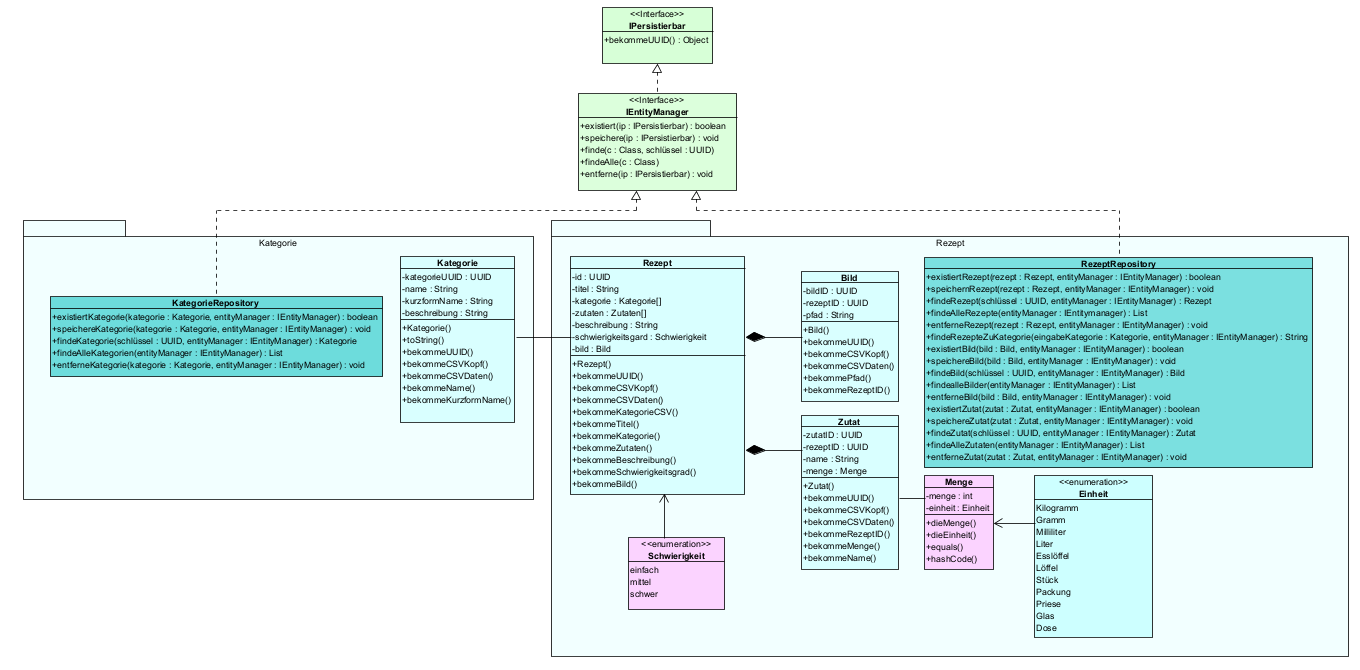
\includegraphics[width=0.90\textwidth]{Bilder/Reposetory-UML.png} 
	\caption{UML-Diagramm Repositories}
	\label{fig:RepositoriesUML}
\end{figure}

\chapter{Clean Architecture}\label{CA}

Dieses Kapitel beschreibt die Architektur der entwickelten Software. Es wurde nach den in der Vorlesung erläuterten Clean-Architecture-Prinzipien gebaut. Clean Architecture ist ein Softwarearchitektur-Muster, welches zum Ziel hat, die Abhängigkeiten innerhalb einer Anwendung zu minimieren und die Wiederverwendbarkeit und Testbarkeit zu maximieren. Es besteht aus einer inneren Schicht von unabhängigen Entitäten, die von einer äußeren Schicht von Abhängigkeiten umgeben sind. Dies ermöglicht es Entwicklern, Anwendungen zu erstellen, die leicht zu testen, zu verstehen und zu warten sind und die flexibel sind, um schnell auf Änderungen reagieren zu können.

Im Folgenden werden die verwendeten Schichten genauer erläutert. Die Schicht \enquote{Abstraction Code} wurde in unserer Anwendung nicht verwendet, da für die in der Domäne behandelten Themengebiete kein Domänen übergreifendes Wissen notwendig war, welches Teil dieser Schicht hätte sein müssen. 
Außerdem haben wir die Adapters-Schicht und die Application Code Schicht vereint, da nicht ausreichend Codesubstrat für beide Schichten vorhanden war. Der Code dieser Schichten befinden sich in der \href{https://github.com/MichaelaHaag/RezeptApp/tree/main/1-Adapter}{\code{Schicht 1: Adapters Code}}.

\section{Schicht 3: Domain Code}
Die \href{https://github.com/MichaelaHaag/RezeptApp/tree/main/3-Domain-Code}{\code{Domain Code Schicht}} umfasst die unabhängigen und wiederverwendbaren Geschäftslogikkomponenten der Anwendung. Sie enthalten keine Abhängigkeiten von anderen Schichten und sind in der Regel unabhängig von der Benutzeroberfläche oder der Datenpersistenz.
Die Domain Code Schicht enthält die beiden Aggregate und die enthaltenen Entitäten und Value Objects der Softwaredomäne. Für beide Aggregate wurde jeweils ein eigenes Repository erstellt, welches sich auch in der Domain Code Schicht befinden. Zudem befindet sich im Domain Code das Interface \href{https://github.com/MichaelaHaag/RezeptApp/tree/main/3-Domain-Code/src/main/java/de/rezeptapp/domain/IEntityManager.java}{\code{IEntityManager}} für die Dependecy Injection. Eine genauere Erläuterung befindet sich in \autoref{DI} Dependency Inversion. Die Interfaces \code{IEntityManager} und \href{https://github.com/MichaelaHaag/RezeptApp/tree/main/3-Domain-Code/src/main/java/de/rezeptapp/domain/IPersistierbar.java}{\code{IPersistierbar}} wurden beide neu erstellt. Alle Entitäten der Domäne, welche gespeichert werden sollen, implementieren das Interface \code{IPersistierbar}. Dieses wird dazu genutzt, um sicherzustellen, dass die Entitäten eine UUID zum Speichern im EntityManager haben.
Der Code in dieser Schicht verwendet nur Java-Standards, sodass er als Kern und langlebigste Softwareschicht keine Abhängigkeiten aufweist. \autoref{fig:DomainCodeUML} zeigt die Domain Code Schicht als UML-Diagramm. 
\begin{figure}[ht]
	\centering
	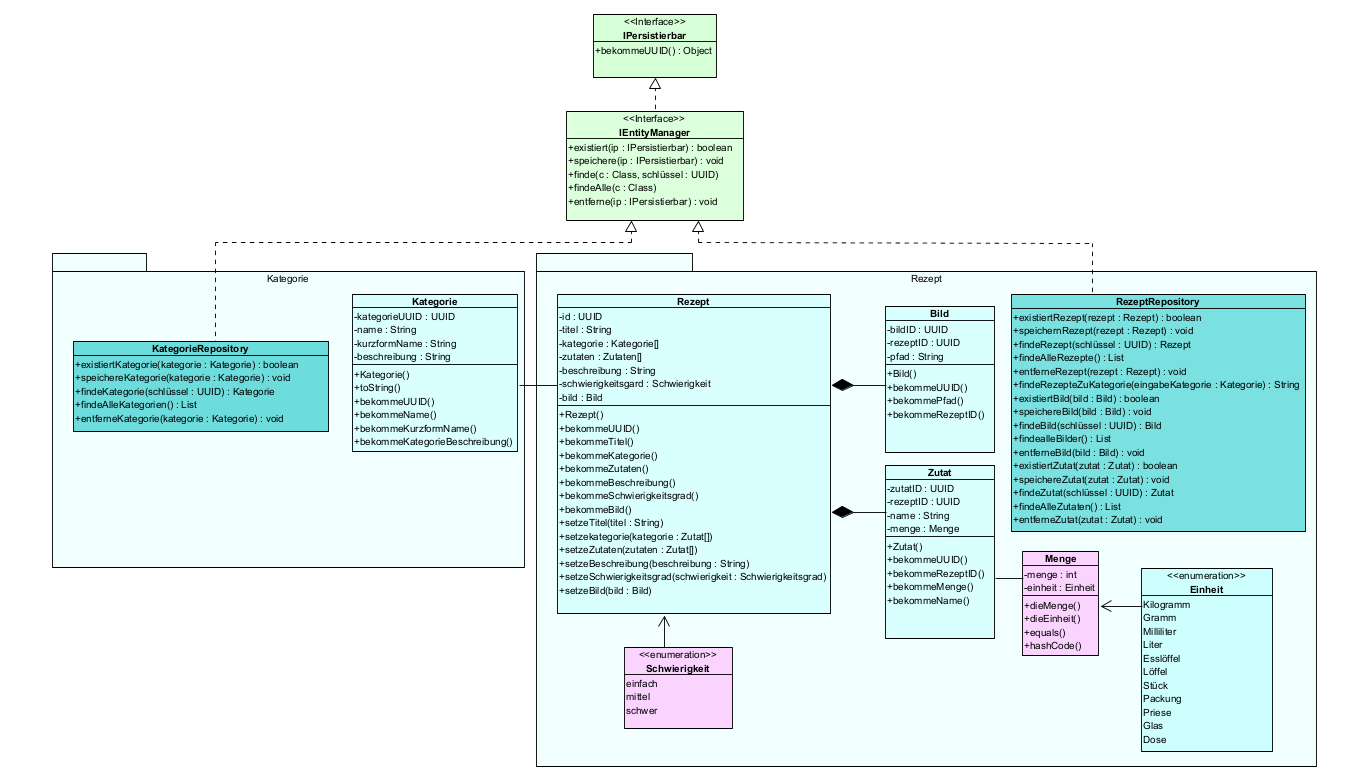
\includegraphics[width=0.90\textwidth]{Bilder/DomainCode-UML.png} 
	\caption{UML-Diagramm Domain Code Schicht}
	\label{fig:DomainCodeUML}
\end{figure}

\section{Schicht 1: Adapters}
Die \href{https://github.com/MichaelaHaag/RezeptApp/tree/main/1-Adapter}{\code{Adapters-Schicht}} in Clean Architecture stellt die Schnittstelle zwischen der Anwendung und externen Systemen dar. Sie ermöglicht die Kommunikation der Anwendung mit der Umgebung und besteht aus Adaptern, die dafür verantwortlich sind, die Daten von der Anwendung in eine Form zu konvertieren, die von den externen Systemen verarbeitet werden kann und umgekehrt. In unserer Anwendung befinden sich in der Adapters-Schicht die Funktionalität für die Speicherung und für die GUI. 

Der \href{https://github.com/MichaelaHaag/RezeptApp/tree/main/1-Adapter/src/main/java/de/rezeptapp/adapter/Datenpersistenz/EntityManager.java}{\code{EntityManager}}, welcher für die Datenhaltung zuständig ist, implementiert nun das Interface \code{IEntityManager} aus der Domain Code-Schicht (siehe \autoref{DI} Dependency Inversion). Darüber hinaus befindet sich in dieser Schicht die Konvertierung der Daten, die für die Speicherung notwendig ist. In dieser Anwendung wurde sich für eine Speicherung der Daten in CSV-Dateien entschieden. Die CSV Funktionalitäten werden möglichst in die äußeren Schichten implementiert, um die Art der Speicherung austauschbar zu gestalten. 
Für die Konvertierung wurde der Ordner \href{https://github.com/MichaelaHaag/RezeptApp/tree/main/1-Adapter/src/main/java/de/rezeptapp/adapter/Datenpersistenz}{\code{Datenpersistenz}} erstellt und das Interface \href{https://github.com/MichaelaHaag/RezeptApp/blob/main/1-Adapter/src/main/java/de/rezeptapp/adapter/Datenpersistenz/ICSVPersistierbar.java}{\code{ICSVPersistierbar}} erstellt. \code{ICSVPersistierbar} wird dazu genutzt, um sicherzustellen, dass die zugrunde liegenden persistierbaren Entitäten eine UUID zum Speichern sowie einen Kopf und Daten für die CSV-Dateien bereitstellen. Außerdem befinden sich im Ordner zu jeder persistierbaren Entität des Domain Codes eine eigene Klasse, die dieses Interface implementiert und somit explizite Funktionalität zur Speicherung in CSV-Dateien beinhaltet (z.B. die Klasse \href{https://github.com/MichaelaHaag/RezeptApp/blob/main/1-Adapter/src/main/java/de/rezeptapp/adapter/Datenpersistenz/CSVZutat.java}{\code{CSVZutat}}). 

Zusätzlich wurde der \href{https://github.com/MichaelaHaag/RezeptApp/tree/main/1-Adapter/src/main/java/de/rezeptapp/adapter/Datenpersistenz/DataReader.java}{\code{DataReader}} implementiert, der die Funktionalitäten zum Laden der Daten aus den CSV-Dateien in den EntityManager und das Speichern in CSV-Dateien beinhaltet. Hierfür erstellt der DataReader die Instanz des \code{EntityManagers} und ruf dann die Funktionalitäten des \code{CSVReader} oder des \code{CSVWriter} auf, welche die Daten laden oder speichern. 

Um die Code-Qualität und Wartbarkeit zu verbessern, wurden die Funktionen, die zuvor in den GUI-Klassen enthalten waren, in separate \href{https://github.com/MichaelaHaag/RezeptApp/tree/main/1-Adapter/src/main/java/de/rezeptapp/adapter/GUIFunktionen}{\code{Funktionen-Klassen}} ausgelagert. Diese Funktionen-Klassen sind nun Teil der Adapters-Schicht, die als Vermittler zwischen der Benutzeroberfläche und den Daten fungiert.


\section{Schicht 0: Plugins}
In der Clean Architecture sind Plugins optional einsetzbare Komponenten, die von der Kernanwendung getrennt sind und über Schnittstellen integriert werden können. Sie ermöglichen es, die Anwendung um zusätzliche Funktionen oder Integrationsmöglichkeiten zu erweitern, ohne die Kernanwendung selbst zu verändern. In unserer Anwendung haben wir die Plugins in \href{https://github.com/MichaelaHaag/RezeptApp/tree/main/0-Plugins}{\code{Plugins}} und \href{https://github.com/MichaelaHaag/RezeptApp/tree/main/0-Plugins-Main}{\code{Plugins-Main}} aufgeteilt.
In den Plugins sind alle GUI-Klassen implementiert.

Die Plugins-Main Schicht beinhaltet die Main Methode zum Starten der App. In der Main-Methode wird die DataReader Instanz instanziiert und die Daten aus den CSV-Dateien geladen, bevor die Startseite gestartet wird. Da die darunter liegenden Schichten aufgrund der Dependency Rule dann nicht mehr auf den DataReader und somit auch nicht auf den EntityManager zugreifen könnten, wird die Instanz des DataReaders an die darunter liegenden Schichten beim Aufruf weitergegeben.


\section{Dependency Inversion}
\label{DI}
In der ursprünglichen Architektur haben Repositories innerhalb der Domain Code Schicht den \code{EntityManager} aus der Adapters-Schicht aufgerufen. Dies verstieß gegen das Prinzip der Dependency Rule, das besagt, dass Abhängigkeiten immer von innen nach außen gerichtet sein sollten.

Um dieses Problem zu beheben, werden die Prinzipien der Dependency Inversion und Dependency Injection eingesetzt, um sicherzustellen, dass der EntityManager in der Domain-Schicht aufgerufen werden kann, ohne die Abhängigkeiten zwischen den Schichten zu verletzen.
Zu diesem Zweck wird das Interface \href{https://github.com/MichaelaHaag/RezeptApp/tree/main/3-Domain-Code/src/main/java/de/rezeptapp/domain/IEntityManager.java}{\code{IEntityManager}}, in der Domain-Schicht erstellt, welches die Methoden des \code{EntityManager} beinhaltet. Der EntityManager selbst wird in die Adapters-Schicht verschoben und implementiert das \code{IEntityManager} Interface. Um sicherzustellen, dass die Repositories auf den EntityManager zugreifen können, wird beim Aufruf des Repositories eine Instanz des \code{EntityManager}-Objekts übergeben. Da der EntityManager nun als IEntityManager-Typ im Repository-Code deklariert ist, kann er auch in der Domain-Schicht aufgerufen werden, ohne die Dependency Rule zu verletzen. Außerdem war hierbei wichtig, dass Entities in Domain Code Schicht \href{https://github.com/MichaelaHaag/RezeptApp/tree/main/3-Domain-Code/src/main/java/de/rezeptapp/domain/IPersistierbar.java}{\code{IPersistierbar}} implementieren, da dies im EntityManager vorausgesetzt wird. 

Durch die Verwendung von Dependency Inversion und Injection wird die Abhängigkeit zwischen der Domain-Schicht und der Adapters-Schicht umgekehrt, sodass die Domain-Schicht unabhängig von der Adapters-Schicht bleibt. Dies verbessert die Flexibilität und Wartbarkeit der Anwendung und ermöglicht es, Komponenten einfach auszutauschen oder zu erweitern, ohne dass dies Auswirkungen auf andere Schichten hat.



\chapter{Entwurfsmuster}
Entwurfsmuster sind bewährte Methoden, um wiederkehrende Probleme in der Softwareentwicklung zu lösen und stellen somit eine Art Blaupause dar, die zur Verbesserung der Struktur, Klarheit und Flexibilität von Software beitragen. Auch in diesem Projekt wurden Entwurfsmuster eingesetzt. Eines dieser Entwurfsmuster soll im nachfolgenden Abschnitt genauer erläutert werden.

\section{Observer Pattern}
In der Rezept-Anwendung wurde vermehrt mit dem Entwurfsmuster Observer-Pattern (Beobachter) gearbeitet. Das Observer-Entwurfsmuster ermöglicht es, Änderungen an einem Objekt den anderen Objekten mitzuteilen, die sich dafür registriert haben. Der Observer gehört zu der Kategorie der Verhaltensmuster. Das Entwurfsmuster besteht aus zwei Hauptkomponenten: dem Observable (Subjekt) und den Observern (Beobachtern). 
Das Subjekt hat einen Zustand, der sich im Laufe der Zeit ändern kann. Die Beobachter registrieren sich beim Subjekt und werden automatisch benachrichtigt, wenn sich der Zustand des Subjekts ändert. Das Observer-Entwurfsmuster ermöglicht es, Objekte lose zu koppeln, da die Observer keine Kenntnis über den Zustand der Objekte haben müssen, auf die sie reagieren. Dies führt zu einer flexibleren und wartungsfreundlicheren Softwarearchitektur.
Im Folgenden wird das Entwurfsmuster anhand eines Beispiels genauer erläutert. 

Ein Anwendungsbeispiel in der Java-API ist das Eventhandling von AWT/Swing. In der entwickelten Anwendungen wurde mit Java Swing gearbeitet, welche einen Observer (Beobachter) zur Verfügung stellt. Java Swing wurde genutzt, um die Benutzeroberfläche in der Java Anwendung zu erstellen. Diese Benutzeroberfläche ist interaktiv. Um auf die Benutzerinteraktionen zu reagieren, stellt Java Swing das Interface Action Listener bereit. Der Action Listener ist in unserer Anwendung der konkrete Observer (Beobachter) und der JButton das konkrete Subjekt. Jeder Swing-Button erbt von AbstractButton Methoden zum An- und Abmelden von Listenern, sowie eine Methode fireActionPerformed() zur Benachrichtigung der entsprechenden Listener. Diese (ActionListerner) müssen die Aktualisierungsmethode actionPerformed(ActionEvent) implementieren.
\begin{figure}[ht]
	\centering
	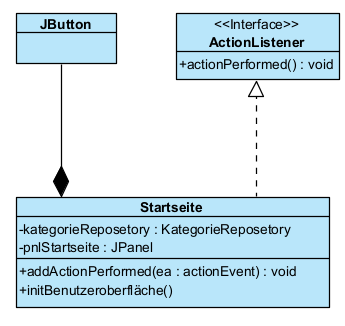
\includegraphics[width=0.70\textwidth]{Bilder/Entwurfsmuster-UML.png} 
	\caption{UML-Diagramm Observer-Pattern Entwurfmuster}
	\label{fig:EntwurfmusterUML}
\end{figure}
\autoref{fig:EntwurfmusterUML} ist das UML-Diagramm unseres Observers am Beispiel der \href{https://github.com/MichaelaHaag/RezeptApp/blob/main/0-Plugins/src/main/java/de/rezeptapp/plugins/gui/Startseite.java}{\code{GUI Startseite}}. 
Auf Grund der Übersichtlichkeit wurden nur die Methoden der Klassen EventListenerList und AbstractButton dargestellt, die für ein besseres Verständnis der Zusammenhänge notwendig sind. 

Der ActionListener in Java hat einige Limitationen. Eine Limitation ist, dass der ActionListener nur für eine Aktion auf einem bestimmten Komponenten-Objekt registriert werden kann, wie z.B. das Klicken auf eine Schaltfläche. Außerdem kann der ActionListener keine Werte zurückgeben, was bedeutet, dass er keine Möglichkeit hat, Feedback oder Informationen an den Aufrufer zurückzugeben, da die Methode actionPerformed vom Typ void ist. Daher kann der ActionListener auch keine Exceptions werfen.
Eine weitere Limitation ist, dass der ActionListener asynchron ausgeführt wird. Er blockiert, bis die Aktion abgeschlossen ist.
Des Weiteren ist ActionListener nur für Mausereignisse geeignet und kann nicht für Tastatureingaben verwendet werden. Dazu kommt, dass der ActionListener nur auf ein einzelnes Mausereignis reagieren kann, wie das Klicken auf eine Schaltfläche oder ein Menüelement. Andere Mausereignisse wie das Bewegen der Maus oder das Drücken der rechten Maustaste werden vom ActionListener nicht akzeptiert. Unser Code arbeitet innerhalb der Limitationen, daher ist der ActionListener für unsere Anwendung gut geeignet. 
\chapter{Programming Principles}
Programming Principles (Programmierprinzipien) sind Grundsätze, die beim Entwurf, der Entwicklung und dem Testen von Software angewendet werden können. Sie sind eine Verallgemeinerung wiederkehrender Erkenntnisse in der Softwareentwicklung und liefern Entwicklern Richtlinien für einen bestimmten Programmierstil.
Im Allgemeinen zielen sie darauf ab, die Qualität und Robustheit von Software zu verbessern. Im folgenden Abschnitt werden drei Programming Principles vorgestellt und deren Anwendung in unserem Projekt analysiert. 

\section{SOLID}
Die SOLID-Prinzipien sind ein Konzept für objektorientierte Programmierung, das fünf Grundsätze für die Entwicklung von hochwertigem und wartbarem Code definiert. Indem man diese Prinzipien befolgt, kann man sicherstellen, dass der Code besser strukturiert und leichter zu erweitern ist, und dass er weniger fehleranfällig ist und besser gewartet werden kann. Jeder Buchstabe in SOLID steht für einen dieser Grundsätze:

\subsection{Single Responsibility Principle (SRP)}
Das Single Responsibility Principle (SRP) besagt, dass ein einzelnes Objekt oder eine Klasse nur für eine einzige Aufgabe oder Verantwortlichkeit zuständig sein  sollte.
In unserer Anwendung ist beispielsweise eine Klasse, die dieses Prinzip strikt einhält: \href{https://github.com/MichaelaHaag/RezeptApp/blob/main/1-Adapter/src/main/java/de/rezeptapp/adapter/GUIFunktionen/FunktionenZufallsGenerator.java}{\code{FunktionenZufallsGenerator}}. Diese Klasse hat lediglich die Aufgabe, aus einer Liste von Rezepten ein \glqq zufälliges\grqq{} Rezept auszuwählen. 
Ein Negativbeispiel für eine Klasse, die das Single Responsibility Principle nicht einhält, ist der \href{https://github.com/MichaelaHaag/RezeptApp/blob/main/1-Adapter/src/main/java/de/rezeptapp/adapter/Datenpersistenz/EntityManager.java}{\code{EntityManager}}. Unser \code{EntityManager} wird verwendet, um eine Verbindung zwischen den Objekten der Anwendung und der zugrunde liegenden Datenbank herzustellen. Mit dem \code{EntityManager} wollten wir die Verwaltung von Objekten und deren Zuständen vereinfachen. Das bedeutet allerdings, dass der \code{EntityManager} mehrere Aufgaben (Verantwortungen), wie das Spichern, Finden, Löschen, etc von Objekten, hat und somit das Prinzip verletzt. 
Andere Positivbeispiele für die Einhaltung des Single Responsibility Principle sind beispielsweise die Klassen \href{https://github.com/MichaelaHaag/RezeptApp/blob/main/1-Adapter/src/main/java/de/rezeptapp/adapter/GUIFunktionen/FunktionenRezeptBearbeiten.java}{\code{FunktionenRezeptBearbeiten}}, \href{https://github.com/MichaelaHaag/RezeptApp/blob/main/1-Adapter/src/main/java/de/rezeptapp/adapter/GUIFunktionen/FunktionenNeuesRezept.java}{\code{FunktionenNeuesRezept}}, \href{https://github.com/MichaelaHaag/RezeptApp/blob/main/1-Adapter/src/main/java/de/rezeptapp/adapter/GUIFunktionen/ButtonRenderer.java}{\code{ButtonRenderer}} und \href{https://github.com/MichaelaHaag/RezeptApp/blob/main/1-Adapter/src/main/java/de/rezeptapp/adapter/GUIFunktionen/FunktionenListenÜbersicht.java}{\code{FunktionenListenÜbersicht}}. Die Klasse \code{FunktionenListenÜbersicht} ist beispielsweise nur dafür verantwortlich alle Rezepte zu einer ausgewählten Kategorie zurückzugeben. 

\subsection{Open-Closed-Prinzip}
Das Open-Closed-Prinzip besagt, dass Software-Entitäten offen für Erweiterungen sein sollten, aber geschlossen bezüglich Veränderungen. Das bedeutet, dass bestehender Code nicht mehr geändert werden sollte, sondern neue Funktionalitäten hinzugefügt werden. Dadurch soll sichergestellt werden, dass die bestehende Funktionalität nicht beeinträchtigt wird und dass die Erweiterung der Software einfacher und sicherer ist. Die Klasse \code{EntityManager}, die auch das Single Responsibility Principle verletzt, ist auch ein Negativbeispiel für das Open-Closed-Principle. Da diese Klasse jeweils alle Use-Cases implementiert, die die Entitytäten betreffen, muss bei geänderten oder neuen Anforderungen diese bestehende Klassen verändert werden.
Ein Beispiel für die Einhaltung des Open-Closed-Principle sind die \href{https://github.com/MichaelaHaag/RezeptApp/blob/main/1-Adapter/src/main/java/de/rezeptapp/adapter/GUIFunktionen}{\code{GUI Funktionen}} in der Adapterschicht.
Hier existiert für jeden einzelnen Use-Case eine separate Klasse, sodass bei neuen Anforderungen lediglich eine neue Klasse implementiert werden müsste und damit der bestehende Code nur erweitert. Die einzige Änderung an bestehendem Code würde in den GUI Klassen stattfinden, da dort neue Events bzw. die zugehörigen Callbacks registriert werden.

\subsection{Liskov Substitution Principle (LSP)}
Das Liskov Substitution Principle besagt, dass es möglich sein muss, Instanzen von Objekten durch ihre Subtypen zu ersetzen, ohne die Korrektheit des Programms zu beeinträchtigen. Kurz gesagt, soll die Ableitungsklasse alle Eigenschaften und Methoden der Basisklasse beibehalten und diese nicht modifizieren oder verletzen. Problematisch kann es sein, wenn Subtypen eine Spezialisierung des Supertypen sind. Ein Beispiel einer Verletzung der Regel: Quadrat wird als Subtyp eines Rechteckes implementiert. Subtypen sind eine Spezialisierung des Supertyps.
In dem vorliegenden Projekt ist keine Vererbungsbeziehung vorhanden, die auf das Liskov Substitution Principle untersucht werden kann, da in keinem Fall von einer eigenen konkreten Klasse geerbt wird, sondern nur von abstrakten Klassen. Beispielsweise bei der Klasse \href{https://github.com/MichaelaHaag/RezeptApp/blob/main/0-Plugins/src/main/java/de/rezeptapp/plugins/gui/Startseite.java}{\code{GUI Startseite}}, ist die Untersuchung auf das Liskov Substitution Principle trivial, da die Subtypen keine Funktionalität des Supertypen überschreiben.

\subsection{Interface-Segregation-Principle (ISP)}
Das Interface-Segregation-Principle besagt, dass mehrere spezifische Interfaces besser sind, als ein Allround-Interface. Die Schnittstellen sollten also schlank und spezifisch sein, damit Clients nur das implementieren müssen, was sie tatsächlich brauchen, anstatt gezwungen zu sein, unnötige Methoden zu implementieren, um Abhängigkeiten und Kopplung zwischen Modulen oder Klassen zu reduzieren und die Wartbarkeit und Flexibilität des Codes zu verbessern.

Gute Beispiele für die Einhaltung des Interface-Segregation-Principles finden sich in den Klassen \href{https://github.com/MichaelaHaag/RezeptApp/blob/main/1-Adapter/src/main/java/de/rezeptapp/adapter/Datenpersistenz/ICSVPersistierbar.java}{\code{ICSVPersistierbar}} und \href{https://github.com/MichaelaHaag/RezeptApp/tree/main/3-Domain-Code/src/main/java/de/rezeptapp/domain/IPersistierbar.java}{\code{IPersistierbar}} wieder.
Beide Interfaces haben jeweils nur eine oder wenige Methode, die nur einen einzigen Nutzen definieren. Das Interface \code{ICSVPersistierbar} enthält Methoden die zur Speicherung der Objekte notwendig sind und in den Objekten implementiert werden müssen. \code{IPersistierbar} wird verwendet, um die UUID zu lesen, die im EntityManager benötigt wird. Für dieses Vorhaben definiert dieses Interface die Methode \code{bekommeUUID}.

Ein Negativbeispiel für die Einhaltung des Interface-Segregation-Principles findet sich in dem Interfaces \code{IEntityManager}. Diese kombiniert jeweils den schreibenden Zugriff, das Löschen und das Suchen von Objekten in einem einzigen Interface. Dieses Interface könnte aufgeteilt werden auf jeweils ein Interface für den schreibenden Zugriff, eins für das Löschen von Objekten und ein weiteres Interface für das Suchen nach Objekten. Dadurch bräuchte ein Client, welcher nur schreibende Zugriffe benötigt, keine Abhängigkeiten auf ein Interface, welches auch löschenden Zugriff erlaubt. Durch eine solche Aufteilung könnte eine Zugriffsverwaltung wesentlich leichter implementiert werden.

\subsection{Dependency-Inversion-Principle (DIP)}
Das Dependency-Inversion-Principle besagt, dass Klassen höherer Ebenen nicht von Klassen niederer Ebenen abhängig sein sollen, sondern beide von Interfaces. Durch die Verwendung von abstrakten Schnittstellen oder Interfaces können Änderungen an einer konkreten Implementierung vorgenommen werden, ohne dass dies Auswirkungen auf die anderen Module oder Klassen hat, die von dieser Implementierung abhängen. Das Dependency-Inversion-Principle trägt somit zur Flexibilität, Erweiterbarkeit und Wartbarkeit von Software bei.
Ein Beispiel für das Dependency-Inversion-Principle ist unser Entity Manager. Hier wurde die allgemeine Schnittstelle \code{IEntityManager} definiert, welches die Methoden des EntityManager beinhaltet. Der EntityManager selbst wird in die Adapters-Schicht implementiert. Dadurch haben die Entitäten im Domain Code keine Abhängigkeit auf die konkreten Implementierungen, sondern erhält diese lediglich durch Aufrufe der Methoden. Ein negatives Beispiel gibt es hier nicht, da die Rezept Anwendung in \autoref{CA} 

\section{GRASP}
GRASP steht für General Responsibility Assignment Software Patterns/Prinziples und ist ein Muster oder Prinzip, dass sich mit der Zuweisung von Verantwortlichkeiten an Objekte befasst. GRASP stellt 9 Lösungsprinzipien für die Softwareentwicklung vor. Zum Grundkonzept gehören zwei der Lösungsprinzipien: Low Coupling und High Cohesion. Beide gehören mit zu den wichtigsten Prinzipen für das GRASP-Programmierprinzip. Daher werden beide im folgenden anhand unserer Anwendung erläutert und analysiert.

\subsection{Low Coupling}
Low Coupling ist eines der Muster, das sich auf die Reduzierung der Abhängigkeiten einer Klasse von ihrer Umgebung konzentriert. Das Ziel ist es, die Verbindungen zwischen den verschiedenen Komponenten im System zu minimieren, um eine höhere Flexibilität, leichtere Anpassbarkeit, gute Testbarkeit, erhöhte Wiederverwendbarkeit und Erweiterbarkeit zu erreichen. Außerdem je loser die Kopplung ist, desto leichter ist die Austauschbarkeit der Funktionalität.
Auch die in \autoref{CA} gemachten Änderungen haben darauf abgezielt die Kopplung zu reduzieren. Denn das Ziel von Clean Architecture ist, die Abhängigkeiten zwischen verschiedenen Schichten eines Systems zu minimieren. Das bedeutet, dass jede Schicht in der Architektur so gestaltet wurde, dass sie nur von den Schichten darunter abhängt und keine Kenntnis über die Schichten darüber hat. Da das Projekt der Clean Architecture entspricht, gilt allgemein, dass die inneren Schichten keine Kopplungen zu den äußeren Schichten haben. 
Somit sollten die Klassen, in der untersten Schicht, im Domain Code, generell eine geringere Kopplung als die Klassen in den Plugins haben. Allerdings können die Klassen in den untern Schichten auch innerhalb einer Schicht viele Abhängigkeiten haben. So haben die Klasse Bild und Schwierigkeit eine geringe Kopplung, wobei Rezept eine hohe Kopplung hat.  
In der Klasse Rezept koppeln sich die Abhängigkeiten mit den Klassen Kategorie, Zutat, Bild und Schwierigkeit. Für eine zusätzliche stärkere Kopplung sorgt die Instanziierung der Arraylisten von Kategorie und Zutat im Konstruktor.
Auf der anderen Seite sind neben einigen Domain-Code Klassen unsere GUI-Klassen Beispiele für Klassen mit schwacher Kopplung. Diese Klassen besitzen jeweils nur wenige Abhängigkeit (Kopplung) zueinander. 
Ein weiteres Beispiel für geringe Kopplung ist die Klasse FunktionenStartseite. Die Klasse weist eine Abhängigkeit mit der Klasse NeueKategorie auf.

\subsection{High Cohesion}
High Cohesion  ist ein Maß für den inneren Zusammenhalt einer Klasse, zeigt wie eng die Methoden und Attribute einer Klasse zusammenarbeiten. Mit anderen Worten, eine Klasse sollte eng miteinander verbundene und verwandte Funktionalitäten enthalten, um eine hohe Kohäsion zu erreichen. 
Die Klasse EntityManager der GUI Funktionen zeugt von geringerer Kohäsion, da hier mehrere Use-Cases in einer Klasse implementiert werden. Der EntityManager dient der Datenhaltung und hat die Aufgaben, Objekte zu speichern/löschen und zu finden. Eine verbesserte Implementierung bietet sich an, indem die einzelnen Operationen separat in Klassen eines Moduls implementiert werden.

FunktionenZufallsGenerator zeigt von hoher Kohäsion, da diese lediglich einen Use-Case behandelt. Diese Klasse hat lediglich die Aufgabe, aus einer Liste von Rezepten ein „zufälliges“ Rezept auszuwählen. Dafür besitzt diese Klasse lediglich die Methode zufälligeRezeptUUID, die diese Logik implementiert. Auch die Klassen CSVReader und CSVWriter zeigen von hoher Kohäsion. Beide Klassen haben drei Methoden die für das Lesen/Schreiben von den CSV Daten notwendig sind. Einen Konstruktor, eine checkFile und die Lese bzw. Schreibe Funktion. 

\section{DRY}\label{DRY}
Das DRY-Prinzip steht für \glqq Don't Repeat Yourself \grqq{} und besagt, dass man eine bestimmte Information oder Funktionalität in einer Software nur an einer Stelle definieren sollte, um Redundanz zu vermeiden. Jeder Wissensaspekt darf nur eine einzige, unzweideutig verbindliche Repräsentation in einem
System besitzen. Das bedeutet, dass man sich bemüht, Code-Duplikationen zu vermeiden und stattdessen wiederverwendbare Komponenten und Funktionen zu schaffen, die an verschiedenen Stellen in der Software verwendet werden können. Auf diese Weise wird der Code einfacher zu warten, zu testen und zu erweitern.
Ein Beispiel für die Einhaltung ist die Methode findeRezepteZuKategorie in dem Rezept Reposetory. Diese Klasse wurde zentral implementiert und definiert und wird von verschiedenen Klassen aufgerufen, um alle Rezepte zu einer Kategorie zu finden. Durch die zentrale Implementierung wird hier Code-Duplikationen vermieden. 

Ein Negativbeispiel für das Nichteinhalten des DRY-Prinzips ist in der Implementierung der GUI Klassen. Alle GUI's haben den selben Footer. Im Footer befinden sich die drei Buttons: Zufallsgenerator, Startseite und Neues Rezept. Dieser Footer der GUI wurde in jeder Klasse implementiert, in der er angezeigt wird und lediglich der Hauptinhalt wird ausgetauscht. Das führt zu einer Dopplung der Informationen. Würden die Entwickler entscheiden beispielsweise den Footer der GUIs ändern zu wollen und beispielsweise den Button Text Startseite durch HomePage ersetzen zu wollen, müsste diese kleine Änderung in 3 Klassen geändert werden. Diese Verletzung des DRY-Prinzips wurde begangen, weil die Seite ohne Designkonzept entwickelt wurde.  

Ein Beispiel für die Einhaltung des DRY-Prinzips ist die Verwendung unser EntityManager. Der EntityManager dient der Datenhaltung und hat die Aufgaben, Objekte zu speichern/löschen und zu finden. Er wird von allen Objekten benutzt und sorgt somit dafür, dass nicht jedes Objekt diese Methoden implementieren muss. 


\chapter{Unit Tests}

Im vorliegenden Projekt wurden Unit Tests eingesetzt, um die Qualität der Software zu sichern und Fehler frühzeitig zu erkennen. Die implementierten Tests konzentrieren sich hauptsächlich auf die Domaincode- und Adapters-Schichten, da hier die Funktionalität des Codes von größter Bedeutung ist. Hier wurden allerdings nur exemplarische Klassen getestet. Für die Peripherie der Software in der Plugin-Schicht wurde zunächst auf Unit Tests verzichtet, da dieser Teil des Programms ohnehin leicht und häufig austauschbar sein soll und daher von geringerer Wichtigkeit ist, sodass ihm auch beim Testen eine geringere Priorität zugewiesen wurde.

Um eine möglichst korrekte Implementierung der Software zu erreichen, wird die AAA-Normalform wird angewendet. Die AAA-Normalform strukturiert jeden Unit Test in drei Bereiche: Arrange (Initialisierung der Testumgebung), Act (Ausführung der zu testenden Aktion) und Assert (Überprüfung der Testergebnisse).

\section{ATRIP-Regeln}

Die ATRIP-Regeln sind fünf grundlegende Regeln für Unit Test, welche verwendet werden, um sicherzustellen, dass die diese klar, verständlich und effektiv sind. In den nachfolgenden Abschnitten wird untersucht, wie sie in diesem Projekt angewendet wurden.

\subsection{Automatic}

Alle implementierten Unit Tests laufen vollständig eigenständig ab, da keinerlei manuelle Eingriffe, etwa in Form von Werteeingaben, notwendig sind. Außerdem überprüfen alle Tests ihre Ergebnisse durch Assertions automatisch, dass diese den im Code eingetragenen erwarteten Ergebnissen entsprechen. Die Tests werden durch JUnit 5 automatisch ausgeführt. Nach dem Durchlaufen eines Testes wird das Testergebnis in \enquote{bestanden} oder \enquote{nicht bestanden} klassifiziert. IntelliJ bestätigt ein erfolgreiches Durchlaufen aller Tests mittels eines grünen Hakens.

\subsection{Thorough}

Bei dieser Regel soll jede missionskritische Funktionalität getestet wird. Jedoch ist eine eindeutige Entscheidung, ob alles Notwendige getestet wurde und damit die Regel erfüllt ist, schwierig. Als „notwendig“ wurde für das vorliegende Projekt die wesentliche Businesslogik und damit die Adapters-Schicht definiert. Diese wird mit einer hohen Testabdeckung (Code Coverage) getestet, sodass die implementierten Tests durchaus als gründlich bezeichnet werden können (vgl. \autoref{CodeCoverage}). Da ohne den Domain-Code nichts funktionieren würde und dieser langfristig so gut wie nie verändert werden soll, wurden hier auch exemplarische Methoden getestet, allerdings nicht sehr ausführlich, da diese Tests sehr ähnlich aufgebaut wären. Allerdings wurden keine Tests für spezifische Softwarefehler implementiert, da sich die Software zum Zeitpunkt der Verfassung noch nicht ausgiebig von Endanwendern getestet wurde und daher bisher keine Softwarefehler gemeldet wurden.

\subsection{Repeatable}

Unter dem Aspekt Repeatable, sollte jeder Unit Test automatisch durchführbar sein und kontinuierlich das gleiche Testergebnis liefern, da sie weder zeit- noch zufallsabhängige Komponenten beinhalten und keine Abhängigkeiten auf Datenbanken oder Dateisystemen haben. Um zuverlässige Tests bei den variablen Komponenten zu ermöglichen, wird auf Mock-Objeckte zurückgegriffen, da sie fortlaufend die gleichen Daten dem Test liefern. (siehe \autoref{Mocks})


\subsection{Independent}

Die Unit Tests müssen jederzeit in beliebiger Reihenfolge ausführbar sein. Dies wird sichergestellt, indem die Unit Tests keine impliziten Abhängigkeiten untereinander besitzen und die AAA-Normalform strikt befolgt wird, also jeder Test in seiner ersten Phase seine eigene „Testwelt“ initialisiert. Im Produktivbetrieb gibt es Abhängigkeiten auf persistierte Daten. Um dieses in den Unit Tests zu verhindern, werden jegliche Persistenzzugriffe auf Mocks ausgeführt, welche in der ersten Phase jedes Tests neu trainiert werden.

\subsection{Professional}

Die Unit Tests sollen eine einheitliche, leicht verständliche Syntax und übersichtliche Struktur vorweisen, um den Umgang und das Weiterentwickeln im professionellen Bereich zu vereinfachen. Durch gleiche Namenskonventionen, die aus der Ubiquitous Language hervorgehen, und der Aufbau der Tests nach der AAA-Normalform wird das Kriterium an diese Regel erfüllt. Zu dem professionellen Standard gehört zudem, dass die Dateinamen und die Programmcodes der Tests verständlich und nachvollziehbar sind. Hierfür hat die Testklasse denselben Namen wie die zu testende Klasse nur mit dem Suffix \enquote{Test}. Bei den Testmethoden gilt dasselbe nur mit dem Präfix \enquote{test\_}. Dadurch soll die Zuordnung der Methoden zu den jeweiligen Unit Tests vereinfacht werden. 


\section{Code Coverage}
\label{CodeCoverage}

Code Coverage ist eine Metrik, die verwendet wird, um den Umfang zu messen, in dem ein Softwareprogramm während der Testausführung getestet wird. Es misst den Prozentsatz der Codezeilen, die im Rahmen des Testverfahrens erfolgreich durchlaufen wurden.
In der Softwareentwicklung wird häufig Gebrauch von der Line Coverage und der Branch Coverage gemacht. Die Line Coverage gibt den Anteil der durchlaufenen Codezeilen von allen möglichen Codezeilen mit ausführbaren Befehlen an. Die Branch Coverage gibt den Anteil der durchlaufenen Abzweigungen (if-Konditionen oder Schleifen) von allen möglichen Abzweigungen an.

\autoref{fig:CodeCoverageBild} zeigt eine Messung der Code Coverage der IDE IntelliJ IDEA für die Anwendung. So beträgt die Line Coverage insgesamt 33\% und die aussagekräftigere Branch Coverage (in der Abbildung, die Spalte \enquote{Block}) sogar 44,8\%. Insgesamt wird bei der Code Coverage solch ein niedriges Ergebnis erreicht, da nur eine geringe Anzahl an exemplarischen Tests erstellt wurde. 
In der Adapters-Schicht ist die Branch Coverage hoch, jedoch ist die Line Coverage niedrig, da vergleichsweise nur sehr wenige Codezeilen getestet wurden. In der Domain-Schicht ist es genau umgekehrt. Hier ist die Line Coverage mit 64\% sehr hoch, da sehr viele Methoden ausführlich getestet wurden, jedoch ist die Branch Coverage deutlich niedriger, da hier weniger Abzweigungen getestet wurden. 

Besonders gut ist dabei das Einhalten der Dependency Rule zu sehen: Da nur die Adapters-Schicht und das Rezept Package des Domain Codes getestet wurden, hat die Plugin-Schicht keinerlei Testabdeckung. Der Domain Code Kategorie, welcher keine eigenen Tests besitzt, ist hingegen zu teilen getestet, da eine Abhängigkeit auf diesen durch die Adapters-Schicht besteht.

\begin{figure}[ht]
	\centering
	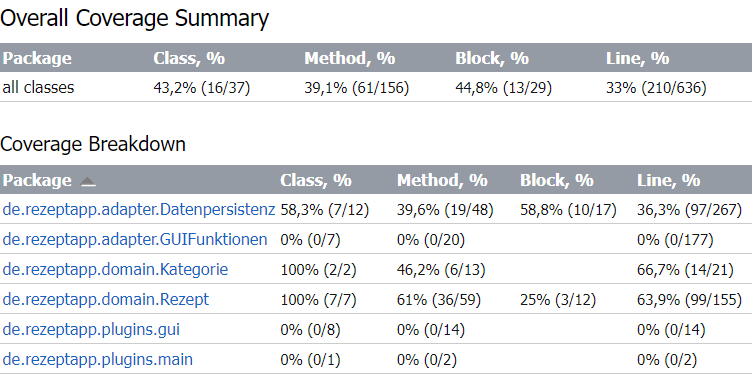
\includegraphics[width=0.90\textwidth]{Bilder/CodeCoverage.png} 
	\caption{Code Coverage der Rezept App}
	\label{fig:CodeCoverageBild}
\end{figure}

\section{Mock-Objekte}
\label{Mocks}

Mock-Objekte (Mocks) werden stellvertretend für reale Softwareobjekte verwendet, um eine Klasse isoliert zu testen. Wie in der Repeatable ATRIP-Regel bereits benannt, ersetzten Mock-Objekte die Abhängigkeiten von Klassen als Objekt mit der für den Unit Test benötigten Funktionalität. Im Rahmen dieses Softwareprojektes wurde auf das Mocking-Framework EasyMock und Testing-Framework JUnit 5 zurückgegriffen.

Verwendet werden die Mock-Objekte in der \emph{RezeptReositoryTest} Klasse. Da hier eine Dependecy Invesion durchgeführt wurde, erhalten alle Methoden als Eingabeparameter ein \emph{IEntityManger}-Objekt. Dieses wird für die Unit Tests durch Mocks ersetzt, welche die für den jeweiligen Test notwendigen Daten liefern. Ein Beispiel für einen Test, welcher ein Mock verwendet ist \emph{test\_findeZutat()}, in welchem der EntityManager gemockt wird. Dazu wird das Mock-Objekt zunächst durch EasyMock erstellt, anschließend trainiert und aktiviert. Im Training wird dem Mock-Objekt beigebracht, auf den Methodenaufruf \emph{finde()} ein bestimmtes Zutat-Objekt zurückzugeben. Abschließend wird überprüft, ob das zurückgegebene Objekt mit dem erwarteten Objekt übereinstimmt und ob das Mock-Objekt richtig verwendet wurde. 

\chapter{Refactoring}
Refaktorisierung (auch als Refactoring bezeichnet) ist ein Prozess in der Softwareentwicklung, bei dem der Code einer Anwendung geändert wird, ohne das Verhalten der Anwendung selbst zu ändern. Das Ziel von Refaktorisierung ist es, den Code zu verbessern, indem er einfacher, verständlicher und wartbarer gemacht wird.

Während der Entwicklung von Software kann es vorkommen, dass der Code mit der Zeit unübersichtlich und komplex wird. Dies kann dazu führen, dass Änderungen oder Erweiterungen an der Software schwierig und fehleranfällig sind. Durch Refaktorisierung kann der Code so umstrukturiert werden, dass er einfacher zu verstehen und zu warten ist.
\subsection{Code Smells}
Code Smells sind Indikatoren für potenzielle Probleme im Code bzw. die Bezeichnung für verbesserungswürdige Codestellen, die bei der Refaktorisierung behoben werden können. 
\subsubsection{Duplicated Code}
Duplicated Code ist ein Code-Smell, bei dem derselbe Code an mehreren Stellen im Programm vorkommt. Das bedeutet, dass eine bestimmte Funktionalität oder Logik mehrmals implementiert wurde, anstatt eine abstrakte Lösung zu entwickeln, die an verschiedenen Stellen im Code wiederverwendet werden kann. In \autoref{DRY} wurden die Stellen an denen Code doppelt existiert schon analysiert. Alle GUI's haben denselben Footer. Im Footer befinden sich die drei Buttons: Zufallsgenerator, Startseite und Neues Rezept. Dieser Footer der GUI wurde in jeder Klasse implementiert, in der er angezeigt wird und lediglich der Hauptinhalt wird ausgetauscht. Das führt zu einer Dopplung der Informationen. Wenn der Entwickler beispielsweise den Footer der GUIs ändern möchte und beispielsweise den Button Text Startseite durch HomePage ersetzen zu wollen, müsste diese kleine Änderung in 3 Klassen geändert werden. 
\subsubsection{Long Method}\label{LM}
Der Code Smell Long Method bezieht sich auf eine lange Methode in einem Programm oder einer Codebasis. Eine lange Methode ist eine Methode, die zu viele Aufgaben ausführt und zu lang ist, um sie leicht zu verstehen, zu warten oder zu ändern. 
Die Methode loadCSVDaten der Klasse \href{https://github.com/MichaelaHaag/RezeptApp/blob/main/1-Adapter/src/main/java/de/rezeptapp/adapter/Datenpersistenz/DataReader.java}{\code{DataReader}} ist vergleichsweise lang. Hier werden die Daten Zeilenweise aus den CSV-Dateien gelesen und im EntityManager gespeichert.
Da es fünf verschiedene CSV-Dateien gibt, muss für jede CSV-Datei ein CSVReader erstellt, die Dateien in eine List gelesen und anschließend jede Zeile auseinander genommen werden. Diese Methode ist aufgrund dessen unlesbar und unübersichtlich. Besser wäre es, dass aufsplitten der einzelnen Zeilen der CSV für jedes Objekt auszulagern. Es wäre sogar denkbar, das Laden der einzelnen CSV-Dateien in eigene Methoden zu packen, um die Funktionalität zu kapseln.
\subsubsection{Large Class}
Der Code Smell Large Class bezieht sich auf eine Klasse in einem Programm, das zu viele Aufgaben hat und zu groß ist, um leicht zu verstehen, zu warten oder zu ändern. Eine große Klasse kann schwer zu lesen und zu verstehen sein, da sie viele Details enthält und nicht in kleinere, leichter zu verstehende Teile aufgeteilt ist. Große Klassen können auch schwer zu warten oder zu ändern sein, da Änderungen an einer großen Klasse Auswirkungen auf viele Teile des Codes haben können. Die Klasse \href{https://github.com/MichaelaHaag/RezeptApp/blob/main/0-Plugins/src/main/java/de/rezeptapp/plugins/gui/RezeptBearbeiten.java}{\code{RezeptBearbeiten}} hat eine stark erhöhte Zeilenanzahl im Vergleich zu anderen Klassen des Projektes. In dieser Klasse wird das Java Swing Frontend implementiert, dass angezeigt wird, wenn ein Benutzer ein vorhandenes Rezept bearbeiten möchte. Hier ist das Single Responsibility Principle verletzt, da die Klasse sowohl das Anzeigen der einzelnen Komponenten implementiert, als auch die Funktionalitäten der einzelnen Buttons. Aufgrund dieser Verletzung des Single Responsibility Principles und der großen Menge an Code ist die Klasse sehr unübersichtlich. Ein weiterer Code Smell Large Class ist die Klasse \href{https://github.com/MichaelaHaag/RezeptApp/blob/main/1-Adapter/src/main/java/de/rezeptapp/adapter/Datenpersistenz/DataReader.java}{\code{DataReader}}. Auch diese Klasse ist verhältnismäßig groß. In dieser Klasse wird die Funktionalitäten zum Laden und Speichern der Daten aus den CSV-Dateien implementiert. Hier ist auch das Single Responsibility Principle verletzt, da die Klasse sowohl das Laden und Speichern der Daten implementiert, aber auch das Erstellen der Objekte aus den geladenen Daten. Aufgrund dieser Verletzung des Single Responsibility Principles und der großen Menge an Code ist die Klasse sehr unübersichtlich. Auch dieser Code Smell sollte behoben werden, indem die Funktionalität in eine weitere Klasse ausgelagert wird.
\subsection{Refactoring}
\subsubsection{Extract Method}
Wie in \autoref{LM} beschrieben, ist die Methode loadCSVDaten sehr lang. Aus diesem Grund wurde hier das Refactoring Extract Method angewendet und somit das aufsplitten der einzelnen Zeilen der CSV für jedes Objekt in eine eigene Methode ausgelagert.
Durch die Auslagerung der Funktionalität wurde der Umfang der Methode reduziert und sie ist übersichtlicher geworden. 
Weiterer Vorteil der Auslagerung ist das die Tests auf die Methode nun einfacher angewendet werden können. 
Dieses Refactoring kann im Commit \href{https://github.com/MichaelaHaag/RezeptApp/commit/d3ace6a38e46831cee35d0b270c41c4fd5783162}{\code{d3ace6a}} eingesehen werden.
\subsubsection{Rename Method}
Das Refactoring Rename Methode musste für unser Projekt nicht angewendet werden, da wir direkt mit den Änderungen der Ubiquitous Language alle Methoden-, Klassen- und Objektnamen in Deutsch und der Domäne entsprechend gewählt haben. Daher haben wir alle Klassen und Methoden Namen so gewählt, dass direkt deutlich wird, was diese Methode macht und wofür eine Klasse zuständig ist.
\subsubsection{Replace Temp with Query}
Das Refactoring Replace Temp with Query zielt darauf ab, die Verwendung von Zwischenvariablen (Temporärvariablen) in Code-Blöcken zu reduzieren oder zu eliminieren, indem sie durch Abfrageausdrücke ersetzt werden. 
Laut Vorlesung sollen temporäre (lokale) Variablen, die zum Zwischenspeichern des Ergebnisses einer Berechnung verwendet werden vermieden werden. Die Berechnungen sollen in einzelne Variablen ausgelagert werden und anschließend sollen Methoden anstatt Variablen gelesen werden. 
Da in unserer Anwendung keine Berechnungen im eigentlichen Sinne betrieben werden, wurden weitere Recherchen zu dem Thema Replace Temp with Query betrieben. Auch Martin Fowler hat das Thema Replace Temp with Query in seinem Buch \glqq Improving the Design of Existing Code \grqq{} beschrieben \footnote[1]{Fowler, Martin: Improving the Design of Existing Code, Addison-Wesley Professional, 1999, S.120 ff.}. So heißt es, dass das Problem mit Temps ist, dass sie temporär und lokal sind. Da sie können nur im Kontext der Methode gesehen werden, in der sie sich befinden verwendet, tendieren Temps dazu, längere Methoden zu fördern. Durch das ersetzten der Temps durch Methoden Aufrufe, kann jede Methode in der Klasse auf die Informationen zugreifen. Das hilft viel dabei, saubereren Code für die Klasse zu entwickeln.
Daher haben wir das Refactoring auf die Methode zufälligesRezeptUUID angewendet. Hierbei wurde keine neue Methode, die die Berechnung durchführt entwickelt, sondern die Anzahl der vorhandenen Temps durch schon vorhandene Methoden zu ersetzen. Der Code-Abschnitt verwendet eine temporäre Variable (zufallsRezept), um ein zufälliges Element aus einer Liste von Rezepten auszuwählen und die UUID dieses Elements zurückzugeben. Stattdessen haben wir die temporäre Variable durch eine direkte Abfrage ersetzt, die die UUID des zufällig ausgewählten Rezepts zurückgibt. Dadurch wurde die Methode übersichtlicher. Die Refaktorisierung können in dem Commit \href{https://github.com/MichaelaHaag/RezeptApp/commit/4e0bedc859ba644d448fe4c89a3a6e1320519593}{\code{4e0bedc}} eingesehen werden. 
Ein weiteres Replace Temp with Query haben wir in der Methode findeRezepteZuKategorie in der Klasse RezeptRepository vorgenommen. Diese Methode sucht alle Rezepte, die zu einer bestimmten Kategorie gehören, und gibt die Daten dieser Rezepte in Form eines String-Arrays zurück. Die Änderungen können in folgendem Commit nachvollzogen werden: 
Der entscheidende Unterschied hier ist, dass die findeAlleRezepte()-Funktion direkt in die Schleife integriert wurde. Das bedeutet, dass die temporäre Variable alleRezepte nicht mehr benötigt wird. Stattdessen wird eine Stream-basierte Abfrage verwendet, um die Kategorien jedes Rezepts abzufragen und zu prüfen, ob die eingabeKategorie darin enthalten ist.
Außerdem wurde die dritte for-Schleife am Ende des ursprünglichen Codes entfernt, die dazu diente, die ausgewähltesRezept-Liste in ein Array umzuwandeln. Stattdessen wurde die toArray()-Methode von ArrayList verwendet, um das Array direkt zu generieren. 
Dadurch wurden in beiden Methoden temporäre Variablen durch Methoden aufrufe ersetzt. Wir haben hier zwar keine neuen Methoden neu erstellt und schon vorhandene Methoden benutzt allerdings konnte trotzdem das Ziel erreicht werden die Klasse zu kürzen und übersichtlicher zu machen. Die gemachten Änderungen können im Commit \href{https://github.com/MichaelaHaag/RezeptApp/commit/4e0bedc859ba644d448fe4c89a3a6e1320519593}{\code{4e0bedc}} eingesehen werden. 

% ---- Literaturverzeichnis
\cleardoublepage
\renewcommand*{\chapterpagestyle}{plain}
\pagestyle{plain}
\pagenumbering{Roman}                   % Römische Seitenzahlen
\setcounter{page}{\numexpr\value{savepage}+1}
\printbibliography[title=Literaturverzeichnis]

% ---- Anhang
\appendix
%\clearpage
%\pagenumbering{Roman}  % römische Seitenzahlen für Anhang

\newpage
\end{document}
